\section{Апробация}

Функциональность сборщика мусора была протестирована на модульных тестах, 
написанных вручную с помощью фреймворка \textbf{googletest}
\footnote{Google Test, Google's C++ test framework,\\ 
\url{https://github.com/google/googletest}}. 
Также было произведено тестирование производительности реализованного алгоритма 
инкрементальной параллельной маркировки. 
Для этой цели использовался известный тест Бёма, активно работающий с динамической памятью. 
В этом тесте строятся двоичные деревья различной глубины с различным количеством узлов. 
Деревья строятся двумя способами: от листов к корню и наоборот, от корня к листьям. 
Было выполнено сравнение библиотеки с аналогами, в частности, с ручным управлением памятью 
с помощью \code{new}/\code{delete}, с классом умного указателя \code{std::shared\_ptr}, 
реализующим подсчёт ссылок, а также с консервативным сборщиком мусора Бёма-Демерса-Вайзера 
c включенной и выключенной опцией инкрементальной маркировки. 
Наша библиотека тестировалась с четырьмя стратегиями: включенной/выключенной 
инкрементальной маркировкой и включенным/выключенным сжатием кучи. 

Измерялось суммарное время работы теста (рис.\ref{fig:boehm}), количество сборок мусора 
(на графике показано как целое число над соответствующим столбцом) и среднее время 
``остановки мира''(рис.\ref{fig:boehm_pause}). 
Все измерения были взяты как среднее и стандартное отклонение по 20 запускам теста. 
Хотя суммарное время работы сборщика с инкрементальной параллельной маркировкой и увеличилось, 
среднее время паузы существенно уменьшились. 
В частности, среднее время паузы при отключенном сжатии при инкрементальной маркировке примерно 
в шесть раз меньше, чем без неё. 
При одновременном включении и сжатия, и инкрементальной маркировки время работы теста 
существенно увеличивается. 
Это объясняется тем, что при инкрементальной маркировки доля объектов, переживающих текущий 
цикл сборки, больше, а время работы текущей реализации процедуры сжатия существенно 
увеличивается при увелечении размера кучи. 
Стоит отметить, что наша библиотека работает примерно в 4 раза медленее чем другие решения, 
участвовавшие в эксперименте, что свидетельствует о необходимости дальнейшей оптимизации.

\begin{figure}[ht!]
\centering
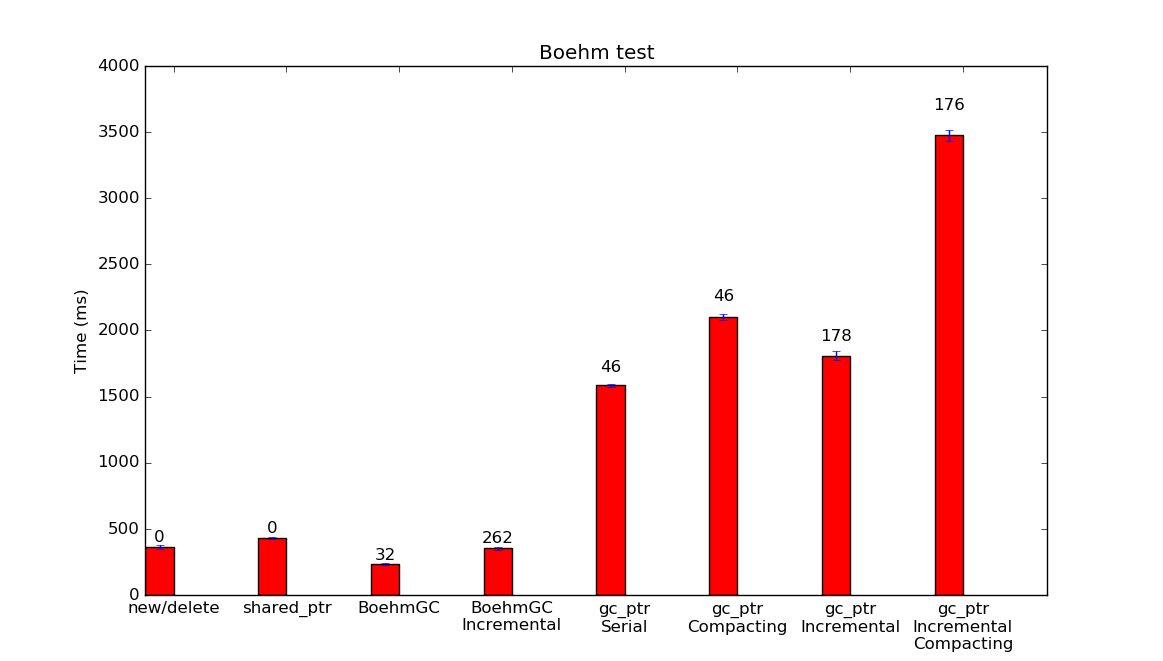
\includegraphics[width=\textwidth]{Moiseenko/images/boehm_all.png}
\caption{Тест Бёма. Суммарное время работы.}
\label{fig:boehm}
\end{figure}

\begin{figure}[h!]
\centering
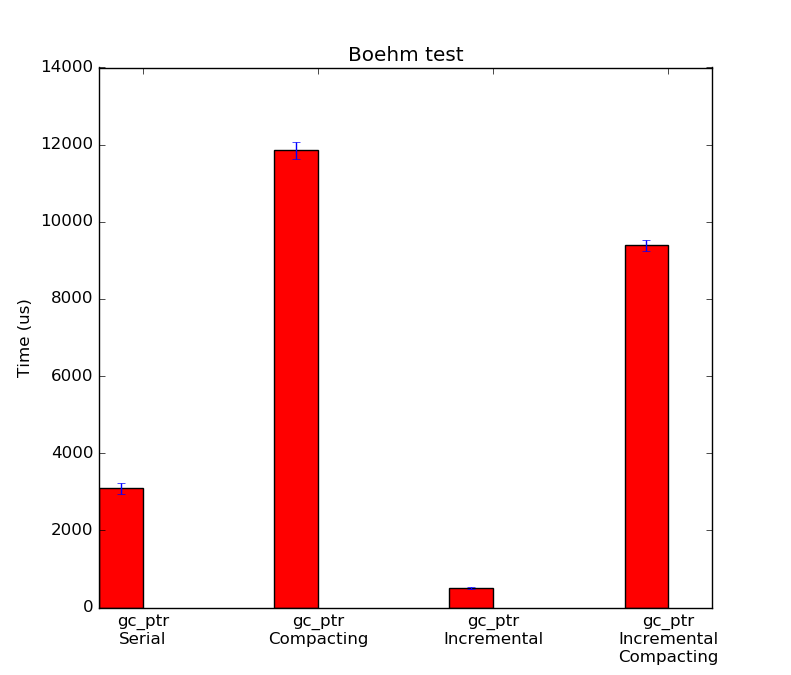
\includegraphics[width=0.8\textwidth]{Moiseenko/images/boehm_pause_all.png}
\caption{Тест Бёма. Среднее время паузы.}
\label{fig:boehm_pause}
\end{figure}

\begin{figure}[h!]
\centering
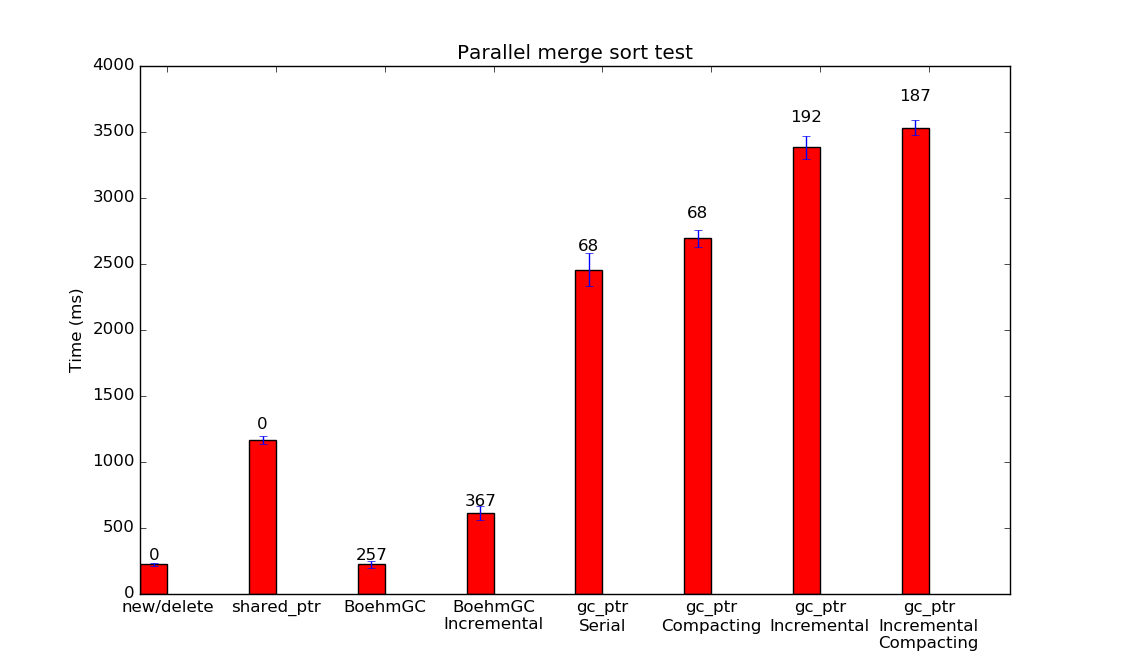
\includegraphics[width=0.8\textwidth]{Moiseenko/images/merge_sort_all.png}
\caption{Многопоточная сортировка слиянием. Суммарное время работы.}
\label{fig:merge_sort}
\end{figure}

\begin{figure}[ht!]
\centering
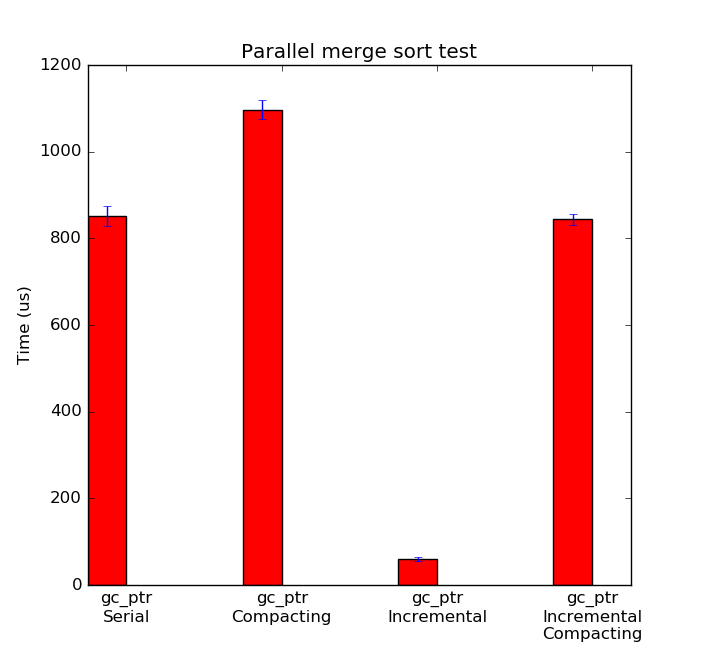
\includegraphics[width=0.7\textwidth]{Moiseenko/images/merge_sort_pause_all.png}
\caption{Многопоточная сортировка слиянием. Среднее время паузы.}
\label{fig:merge_sort_pause}
\end{figure}

Также было протестирована работа сборщика с многопоточным приложением. 
Для этой цели был написан тест, использующий алгоритм сортировки слиянием. 
В этом тесте генерируются односвязные списки. 
Каждый узел списка содержит одно случайное значение типа \code{int}. 
Список разделяется на несколько частей (по числу доступных ядер процессора), 
каждая часть сортируется в отдельном потоке сортировкой слиянием, 
затем части сливаются в единый список. 
Результаты замеров работы библиотеки, а также аналогов, на этом тесте представлены 
на рис.\ref{fig:merge_sort} и рис.\ref{fig:merge_sort_pause}. 
Видно, что результаты данного теста в целом повторяют результаты теста Бёма. 